%!TEX root = ../paper.tex

\begin{sidewaysfigure*}
\subfloat[\textbf{Application:} Average End-to-End Delay]%
{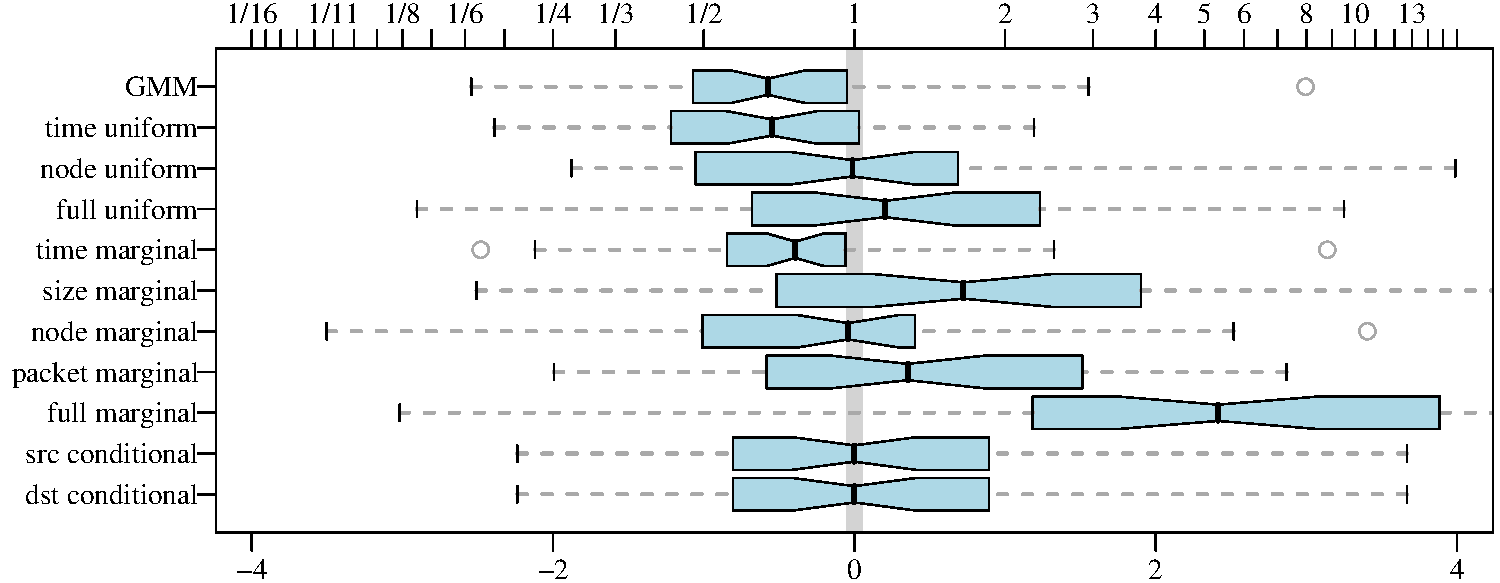
\includegraphics[width=4.5in]{Application/delay.pdf}}\hfill
\subfloat[\textbf{Application:} Packet Delivery Ratio]%
{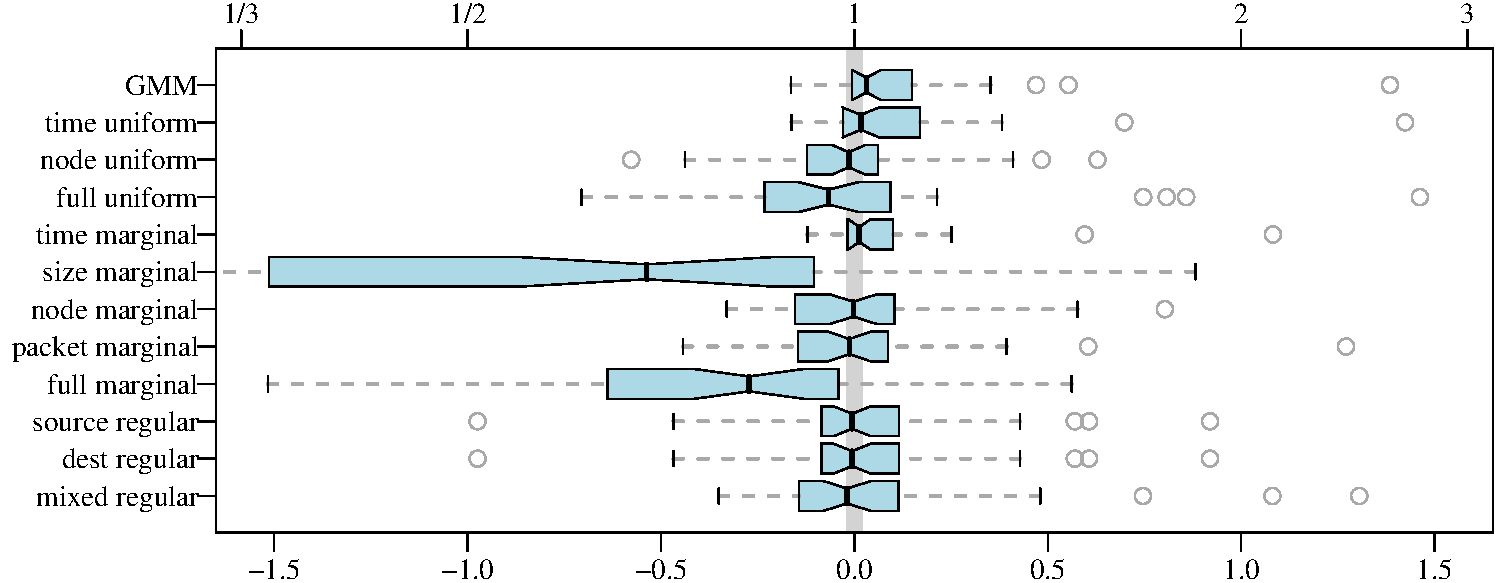
\includegraphics[width=4.5in]{Application/delivery_ratio.pdf}}
%
\subfloat[\textbf{Application:} Average Received Throughput]%
{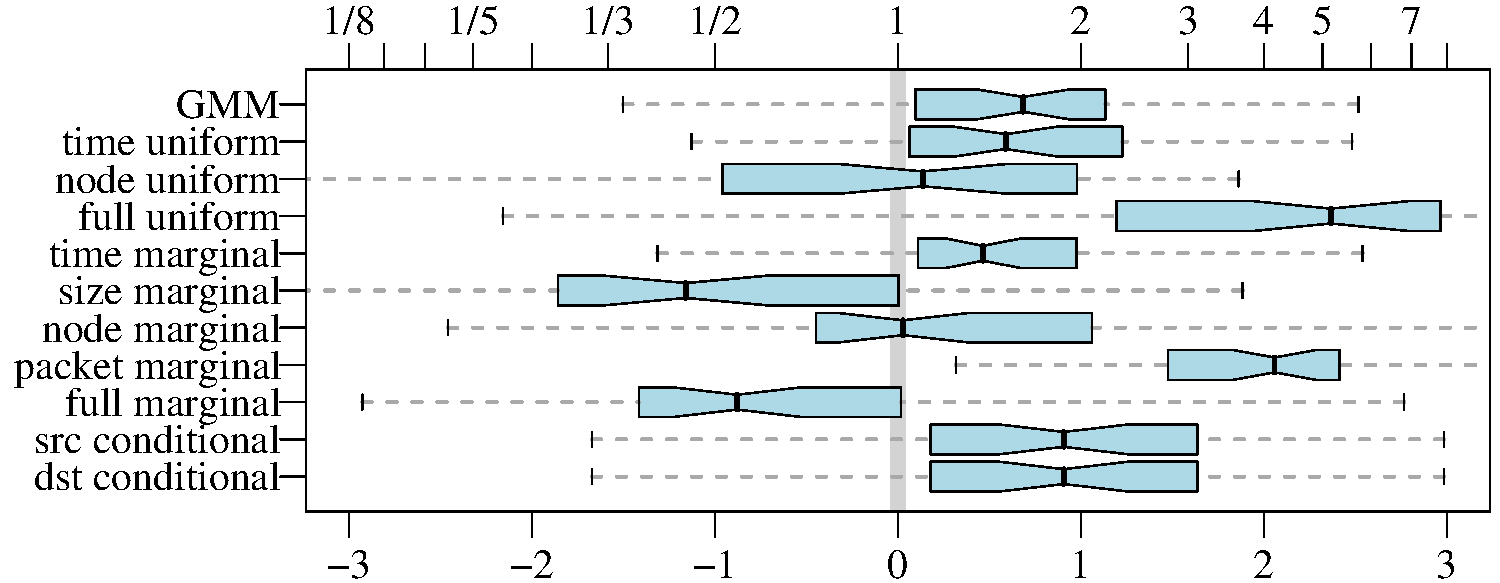
\includegraphics[width=4.5in]{Application/throughput.pdf}}\hfill
\subfloat[\textbf{Network:} AODV Control Overhead]%
{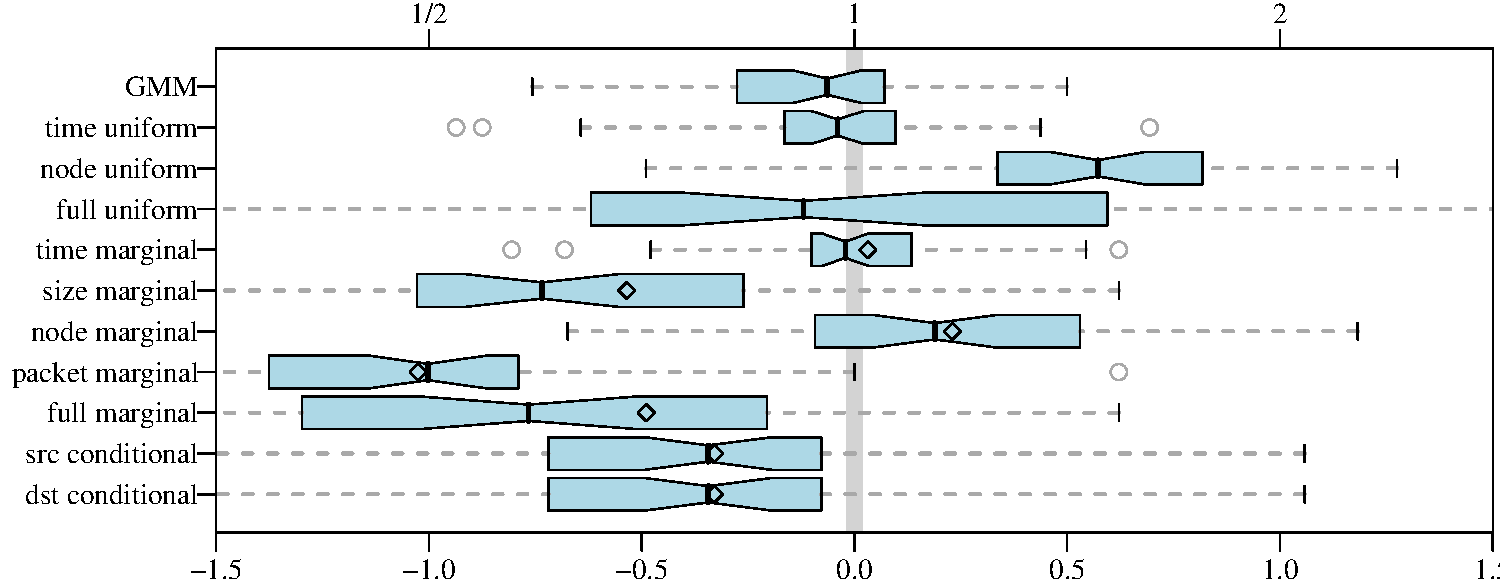
\includegraphics[width=4.5in]{Network/control_packets.pdf}}
%
\subfloat[\textbf{Network:} Packets Dropped in Routing Queue]%
{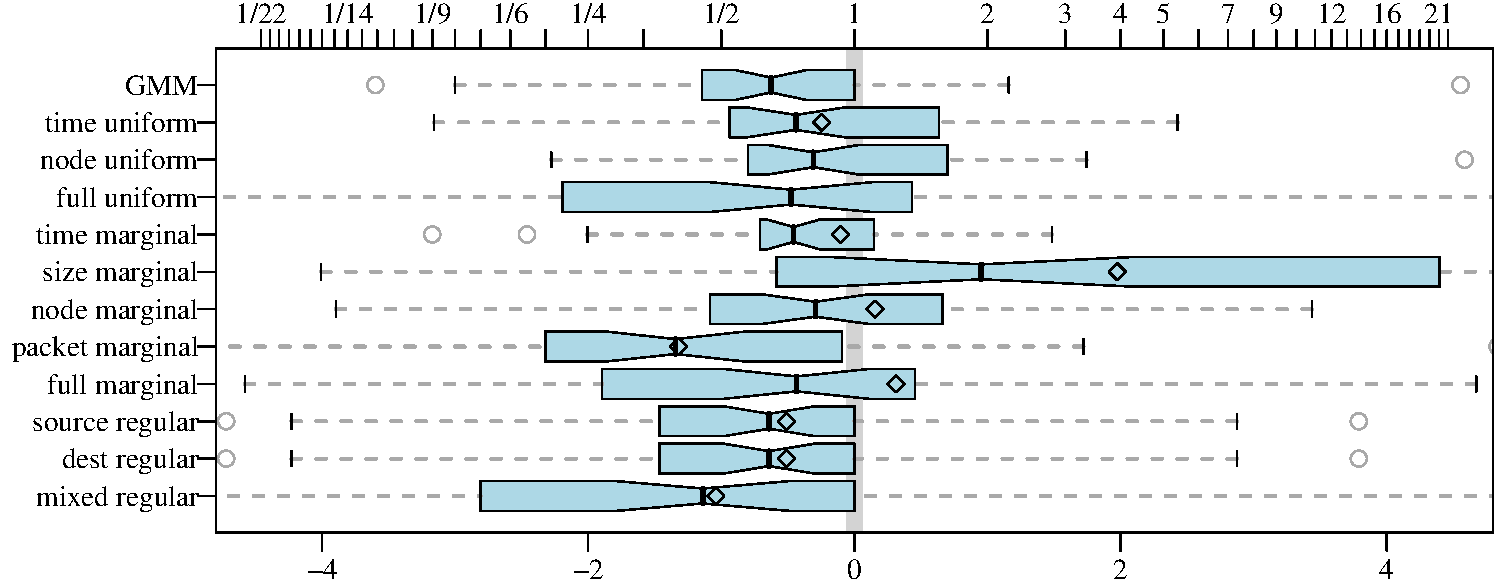
\includegraphics[width=4.5in]{Network/dropped.pdf}}\hfill
\subfloat[\textbf{Link:} 802.11 Control Overhead]%
{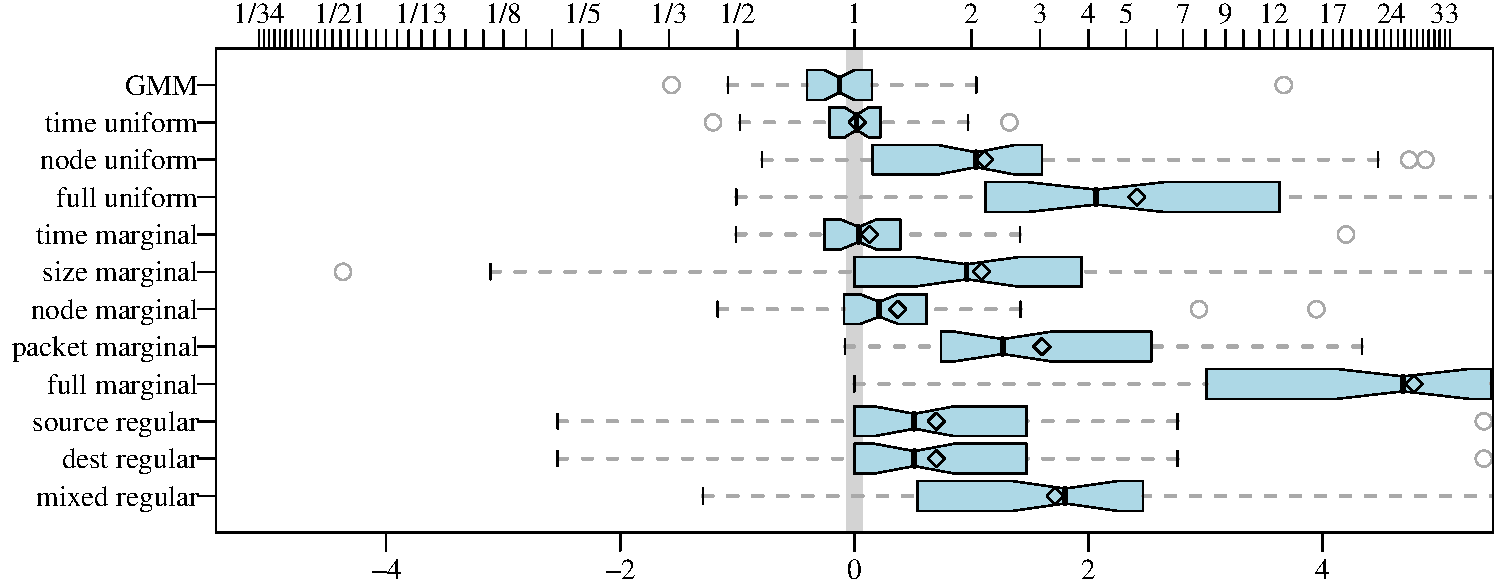
\includegraphics[width=4.5in]{Link/overhead.pdf}}%
%
\caption{%
Box-and-whisker plots of log-ratio error values for all metrics and traffic models.
The lower axis indicates the log-ratio, while the upper axis shows raw ratio values.
Each box contains the central majority of log-ratio values:
the left and right bounds are at the $25^\text{th}$ and $75^\text{th}$ percentiles.
The dark middle line indicates the median value, while the diamond marks the mean.
The whiskers (dotted lines) extend to the furthest non-outlier values, while the points beyond that are outliers. The notch in the middle of each bar indicates a $95\%$ confidence interval for the true underlying median value;
if two notches do not overlap, they are very unlikely to have the same median.
}
\label{fig:box-plots}
\end{sidewaysfigure*}
